\documentclass[a4papper,12pt]{article}
\usepackage{etex}
\reserveinserts{28}

\usepackage{xkeyval}[2005/11/25]
\usepackage{eso-pic}
\usepackage{graphicx}
\usepackage{fp}
\usepackage{tikz}
\usetikzlibrary{calc}
\usetikzlibrary{decorations.pathmorphing}
\usetikzlibrary{decorations.pathreplacing} 
\usetikzlibrary{decorations.shapes} 
\usetikzlibrary{shadows}
\usetikzlibrary{arrows}
\usetikzlibrary{shapes,snakes,shapes.geometric,shapes.misc}
\usepackage{multicol}
\usepackage{arabtex}
\usepackage{amsmath,amsfonts,amssymb}
\usepackage{float}
\usepackage{array,booktabs ,tabularx,multirow}
\usepackage{euler}
\usepackage[top=1cm,bottom=0cm,left=1cm,right=1cm]{geometry}
\usepackage{fancyhdr}
\usepackage{xlop}
\usepackage[most]{tcolorbox}
%----------------------------------------...les compteurs..... ----------------------------------------------------------------------%
\newcounter{i}
\setcounter{i}{1}
\newcounter{k}
\setcounter{k}{1}
%----------------------------------------------------------\cadre[x=... ,y=.....,  ]------------------------------------------------------%

% \cadre[			shadow (bool�en),
%					lw = , (�paisseur du trait, en pt)
%					style = , (dashed ou dotted)
%					x = abscisse du sommet en bas � gauche,
%					y = ordonn�e du sommet en bas � gauche,
%					xshadow = d�calage selon x de l'ombre,
%					yshadow = d�calage selon y de l'ombre,
%					color = couleur du cadre,
%					colorshadow = couleur de l'ombre,
%					decoration = nom de la d�coration,
%					doubleline (bool�en) pour pstricks
%				  ]
\makeatletter
\define@cmdkey [PAS] {cadre} {x}{}
\define@cmdkey [PAS] {cadre} {y}{}
\define@cmdkey [PAS] {cadre} {decoration}{}
\define@cmdkey [PAS] {cadre} {shape}{}
\define@cmdkey [PAS] {cadre} {lw}{}
\define@cmdkey [PAS] {cadre} {xshadow}{}
\define@cmdkey [PAS] {cadre} {yshadow}{}
\define@cmdkey [PAS] {cadre} {bordercolor}{}
\define@cmdkey [PAS] {cadre} {incolor}{}
\define@cmdkey [PAS] {cadre} {shadowcolor}{}
\define@cmdkey [PAS] {cadre} {style}{}
\define@boolkey[PAS] {cadre} {shadow}[true]{}
\define@boolkey[PAS] {cadre} {doubleline}[true]{}

\presetkeys    [PAS] {cadre} {	shadow = false,
								lw = 2,
								x = 0.2,
								y = 0.2,
								xshadow =- 0.35,
								yshadow =0.2,
								bordercolor = black,
								incolor = white,
								shadowcolor = gray,
								style = ,
								doubleline = false,
								decoration = , 
								shape = }{}

\newcommand*{\cadre}[1][]{\pasCadre[#1]}

\def\pasCadre[#1]{
	\setkeys[PAS]{cadre}{#1}
	
	\AddToShipoutPicture
	{
		\put(\LenToUnit{\cmdPAS@cadre@x cm},\LenToUnit{\cmdPAS@cadre@y cm})
		{
				\ifPAS@cadre@doubleline
					\edef\dl{double}
				\else
					\edef\dl{}
				\fi
				\begin{tikzpicture}[decoration={\cmdPAS@cadre@decoration,shape=\cmdPAS@cadre@shape}]
					\pgfsetlinewidth{\cmdPAS@cadre@lw pt}
					\ifPAS@cadre@shadow
						\filldraw[
						decorate,
						fill=\cmdPAS@cadre@incolor,
						draw=\cmdPAS@cadre@bordercolor,
						style=\cmdPAS@cadre@style,
						drop shadow={fill=\cmdPAS@cadre@shadowcolor,shadow xshift=\cmdPAS@cadre@xshadow cm,shadow yshift=-\cmdPAS@cadre@yshadow cm},
						\dl] (0,0) -- (0,\paperheight-2*\cmdPAS@cadre@y cm) -- (\paperwidth-2*\cmdPAS@cadre@x cm,\paperheight-2*\cmdPAS@cadre@y cm) -- (\paperwidth-2*\cmdPAS@cadre@x cm,0) -- cycle;
					\else
						\filldraw[
						decorate,
						fill=\cmdPAS@cadre@incolor,
						draw=\cmdPAS@cadre@bordercolor,
						style=\cmdPAS@cadre@style,
						\dl] (0,0) -- (0,\paperheight-2*\cmdPAS@cadre@y cm) -- (\paperwidth-2*\cmdPAS@cadre@x cm,\paperheight-2*\cmdPAS@cadre@y cm) -- (\paperwidth-2*\cmdPAS@cadre@x cm,0) -- cycle;
					\fi
				\end{tikzpicture}
		}
	}
}

\def\nocadre{\ClearShipoutPicture}
%-----------------------------------------------\entete---------------------------------------------------------------------------%
\newcommand{\entete}{
\noindent
\begin{tabularx}{\textwidth}{|r  ||||X|||| r |}
\toprule
\RL{AlmdT AlzmnyT : sA`tAn}
&
\centering \RL{{\LARGE Al-'imt.hAn Al|m|.hly Al|m|w.hd }}
&
 \RL{_tAnwyT `bd Alkrym Alx.tAby Al-'i`dAdyT}\\
 \RL{AldwrT : $II$}& \centering   \RL{\Large{fy m|AdT AlryA.dyAt}}&\RL{nyAbT tAwryrt} \\
 \RL{Alm`Aml : $3$} & \centering  \RL{AlsnT Al_tAl_tT 'i`dAdy} & \RL{dabdw}\\
 \bottomrule
\end{tabularx}
}
%--\exercice[bareme,bar=...]{........}------------------------------%
\define@cmdkey[EX]{exo}{bar}{}
\define@boolkey[EX]{exo}{bareme}[true]{}
\presetkeys[EX]{exo}{bar= ,bareme=false}{}
\newcommand{\exercice}[2][]{
\setkeys[EX]{exo}{#1}
\setcounter{k}{1}
\tikzstyle{mybox} = [ draw, very thick,rounded corners=3mm, inner sep=10pt, inner ysep=10pt]
\tikzstyle{fancytitle} =[fill=white, text=black,inner ysep=0pt,inner xsep=2pt]
\noindent
\begin{tikzpicture}
\node [mybox] (box){%
    \begin{minipage}{0.88\linewidth}
        #2 
    \end{minipage}
};
\node[fancytitle, left=10pt] at (box.north east) {{\large \arabic{i}\RL{Altmryn}}};
\ifEX@exo@bareme
\node[fancytitle] at (box.north){\RL{nq.t} \cmdEX@exo@bar };
\fi
\end{tikzpicture}%
\stepcounter{i}
}
%-----------\question[bareme,bar=...]{......}----------------------%
\define@cmdkey[EX]{qst}{bar}{}
\define@boolkey[EX]{qst}{bareme}[true]{}
\presetkeys[EX]{qst}{bar= ,bareme=false}{}
\newcommand{\question}[2][]{
\setkeys[EX]{qst}{#1}
\ifEX@qst@bareme
	\ifdim \cmdEX@qst@bar pt  < 2 pt
\begin{arabtext}
$-\arabic{k}$ \marginpar{ \cmdEX@qst@bar{} pt} #2
\end{arabtext}
	\else
\begin{arabtext}
$-\arabic{k}$ \marginpar{ \cmdEX@qst@bar{} pts} #2
\end{arabtext}
	\fi
\else
\begin{arabtext}
$-\arabic{k}$ #2
\end{arabtext}
\fi
\stepcounter{k}
}
%----------\devoir[niv=... , num=..., date=..., ds=...]----------%
\define@boolkey[EX]{devoir}{ds}[true]{}
\define@cmdkey[EX]{devoir}{niv}{}
\define@cmdkey[EX]{devoir}{num}{}
\define@cmdkey[EX]{devoir}{date}{}
\presetkeys[EX]{devoir}{niv=$3$,num=$1$,ds=true,date=}{}
\newcommand{\devoir}[1][]{
\setkeys[EX]{devoir}{#1}

\begin{tikzpicture}
\node [draw,shape=chamfered rectangle] (box1){%
    \begin{minipage}{0.2\textwidth}
      \center \cmdEX@devoir@date \RL{AltAryx :{} }
    \end{minipage}
};
\end{tikzpicture}%
\ifEX@devoir@ds
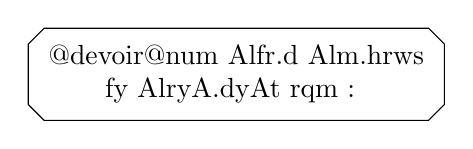
\begin{tikzpicture}
\node [draw,shape=chamfered rectangle] (box2){%
    \begin{minipage}{0.4\textwidth}
       \center\cmdEX@devoir@num \RL{Alfr.d Alm.hrws fy AlryA.dyAt rqm :{} }
    \end{minipage}
};
\end{tikzpicture}%
\else
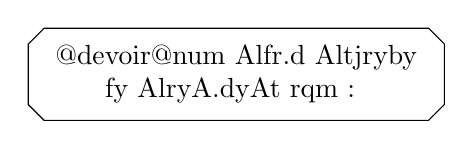
\begin{tikzpicture}
\node [draw,shape=chamfered rectangle] (box2){%
    \begin{minipage}{0.4\textwidth}
       \center\cmdEX@devoir@num \RL{Alfr.d Altjryby fy AlryA.dyAt rqm :{} }
    \end{minipage}
};
\end{tikzpicture}%
\fi
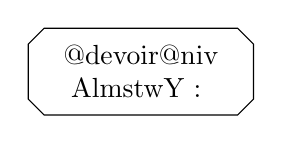
\begin{tikzpicture}
\node [draw,shape=chamfered rectangle] (box3){%
    \begin{minipage}{0.2\textwidth}
 \center\cmdEX@devoir@niv \RL{AlmstwY :{} }     
    \end{minipage}
};
\end{tikzpicture}%
}
%------------------------------------------------\serie[titre=..]-----------------------------------------------------------------------------%

\define@cmdkey[EX]{serie}{titre}{}
\presetkeys[EX]{serie}{titre=\RL{`nwAn Aldrs}}{}
\newcommand{\serie}[1][]{
\setkeys[EX]{serie}{#1}
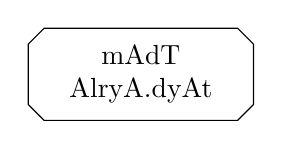
\begin{tikzpicture}
\node [draw,shape=chamfered rectangle] (box1){%
    \begin{minipage}{0.20\textwidth}
       \center\RL{mAdT AlryA.dyAt}
    \end{minipage}
};
\end{tikzpicture}%
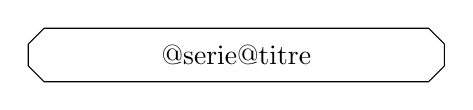
\begin{tikzpicture}
\node [draw,shape=chamfered rectangle] (box2){%
    \begin{minipage}{0.40\textwidth}
      \center\cmdEX@serie@titre
    \end{minipage}
};
\end{tikzpicture}%
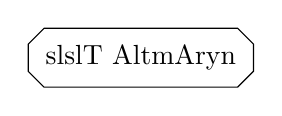
\begin{tikzpicture}
\node [draw,shape=chamfered rectangle] (box3){%
    \begin{minipage}{0.20\textwidth}
   \center\RL{slslT AltmAryn}
    \end{minipage}
};
\end{tikzpicture}%
}
\makeatother

\begin{document}
\devoir[num=6,niv=1,ds=\RL{Almnzly},date=15/05/2017]

\exercice{
\begin{arabtext}
.hdid AlmsA.hT AljAnbyT w .hjm AlmjsmAt AltAlyT
\end{arabtext}
\definecolor{cqcqcq}{rgb}{0.75,0.75,0.75}
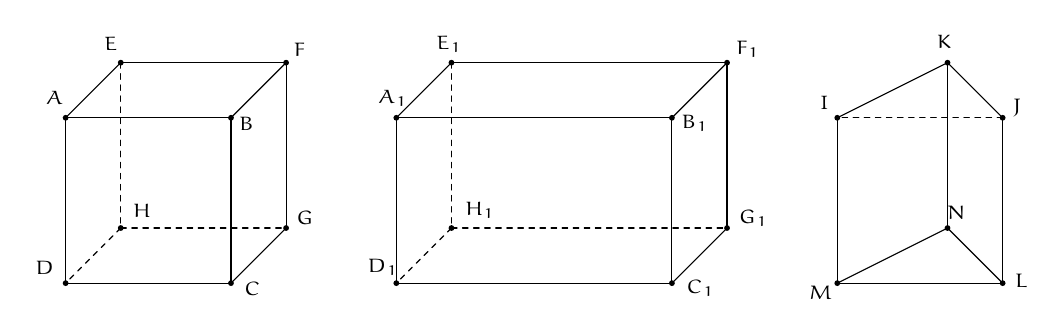
\begin{tikzpicture}[line cap=round,line join=round,>=triangle 45,x=1.0cm,y=1.0cm,scale=0.7]
\draw (-2,4)-- (1,4);
\draw (1,4)-- (1,1);
\draw (1,1)-- (-2,1);
\draw (-2,1)-- (-2,4);
\draw (-1,5)-- (2,5);
\draw (2,5)-- (2,2);
\draw (2,2)-- (1,1);
\draw (1,4)-- (2,5);
\draw (-1,5)-- (-2,4);
\draw [dash pattern=on 2pt off 2pt] (-1,5)-- (-1,2);
\draw [dash pattern=on 2pt off 2pt] (-1,2)-- (-2,1);
\draw [dash pattern=on 2pt off 2pt] (-1,2)-- (2,2);
\draw (4,4)-- (9,4);
\draw (9,4)-- (9,1);
\draw (9,1)-- (4,1);
\draw (4,1)-- (4,4);
\draw (5,5)-- (10,5);
\draw (10,5)-- (10,2);
\draw (10,2)-- (9,1);
\draw (9,4)-- (10,5);
\draw (5,5)-- (4,4);
\draw [dash pattern=on 2pt off 2pt] (5,5)-- (5,2);
\draw [dash pattern=on 2pt off 2pt] (5,2)-- (4,1);
\draw [dash pattern=on 2pt off 2pt] (5,2)-- (10,2);
\draw [dash pattern=on 2pt off 2pt] (15,4)-- (12,4);
\draw (12,4)-- (14,5);
\draw (14,5)-- (15,4);
\draw (15,4)-- (15,1);
\draw (15,1)-- (12,1);
\draw (12,1)-- (12,4);
\draw (12,1)-- (14,2);
\draw (14,2)-- (15,1);
\draw (14,5)-- (14,2);
\begin{scriptsize}
\fill [color=black] (-2,4) circle (1.5pt);
\draw[color=black] (-2.2,4.36) node {$A$};
\fill [color=black] (1,4) circle (1.5pt);
\draw[color=black] (1.28,3.9) node {$B$};
\fill [color=black] (1,1) circle (1.5pt);
\draw[color=black] (1.38,0.9) node {$C$};
\fill [color=black] (-2,1) circle (1.5pt);
\draw[color=black] (-2.38,1.28) node {$D$};
\fill [color=black] (-1,5) circle (1.5pt);
\draw[color=black] (-1.18,5.34) node {$E$};
\fill [color=black] (2,5) circle (1.5pt);
\draw[color=black] (2.24,5.24) node {$F$};
\fill [color=black] (2,2) circle (1.5pt);
\draw[color=black] (2.34,2.18) node {$G$};
\fill [color=black] (-1,2) circle (1.5pt);
\draw[color=black] (-0.62,2.32) node {$H$};
\fill [color=black] (4,4) circle (1.5pt);
\draw[color=black] (3.94,4.36) node {$A_1$};
\fill [color=black] (9,4) circle (1.5pt);
\draw[color=black] (9.42,3.9) node {$B_1$};
\fill [color=black] (9,1) circle (1.5pt);
\draw[color=black] (9.52,0.9) node {$C_1$};
\fill [color=black] (4,1) circle (1.5pt);
\draw[color=black] (3.76,1.28) node {$D_1$};
\fill [color=black] (5,5) circle (1.5pt);
\draw[color=black] (4.96,5.34) node {$E_1$};
\fill [color=black] (10,5) circle (1.5pt);
\draw[color=black] (10.38,5.24) node {$F_1$};
\fill [color=black] (10,2) circle (1.5pt);
\draw[color=black] (10.48,2.18) node {$G_1$};
\fill [color=black] (5,2) circle (1.5pt);
\draw[color=black] (5.52,2.32) node {$H_1$};
\fill [color=black] (12,4) circle (1.5pt);
\draw[color=black] (11.76,4.28) node {$I$};
\fill [color=black] (15,4) circle (1.5pt);
\draw[color=black] (15.26,4.2) node {$J$};
\fill [color=black] (14,5) circle (1.5pt);
\draw[color=black] (13.94,5.38) node {$K$};
\fill [color=black] (15,1) circle (1.5pt);
\draw[color=black] (15.34,1.04) node {$L$};
\fill [color=black] (12,1) circle (1.5pt);
\draw[color=black] (11.7,0.82) node {$M$};
\fill [color=black] (14,2) circle (1.5pt);
\draw[color=black] (14.16,2.28) node {$N$};
\end{scriptsize}
\end{tikzpicture}
}

\exercice{
\begin{minipage}{0.6\linewidth}
\definecolor{xdxdff}{rgb}{0.49,0.49,1}
\begin{tikzpicture}[line cap=round,line join=round,>=triangle 45,x=1.0cm,y=1.0cm]
\draw[->,color=black] (-2.32,0) -- (7,0);
\foreach \x in {-2,-1,1,2,3,4,5,6,7}
\draw[shift={(\x,0)},color=black] (0pt,2pt) -- (0pt,-2pt);
\clip(-2.32,-1) rectangle (7,1.04);
\draw (-1.38,-0.1) node[anchor=north west] {-2};
\draw (-0.28,-0.1) node[anchor=north west] {-1};
\begin{scriptsize}
\fill [color=xdxdff] (2,0) circle (1.5pt);
\draw[color=xdxdff] (2.16,0.4) node {$A$};
\fill [color=xdxdff] (5,0) circle (1.5pt);
\draw[color=xdxdff] (5.18,0.38) node {$B$};
\fill [color=xdxdff] (-2,0) circle (1.5pt);
\draw[color=xdxdff] (-1.86,0.34) node {$C$};
\fill [color=xdxdff] (-1,0) circle (1.5pt);
\draw[color=xdxdff] (-0.84,0.28) node {$D$};
\fill [color=xdxdff] (0,0) circle (1.5pt);
\draw[color=xdxdff] (0.16,0.28) node {$E$};
\end{scriptsize}
\end{tikzpicture}
\end{minipage}
\begin{minipage}{0.4\linewidth}
\begin{arabtext}
.hdid 'afA.syl Alnq.t $A$ w $B$w$C$
\end{arabtext}
\end{minipage}

\begin{arabtext}
m_tl Alnq.t Alm`rfT bAljdwl fy m`lm mt`Amd 'a.slh $O$
\end{arabtext}
\begin{center}
\begin{tabular}{|c|c|c|c|c|c|c|}
\hline 
A & B & E & F & M & D & \RL{Alnq.tT} \\ 
\hline 
-2 & 3 & -1 & 0 & 4 & -2 & \RL{Al-'uf.swl} \\ 
\hline 
0 & 3 & -2 & -4 & 0 & -2 & \RL{Al-'urtwb} \\ 
\hline 
\end{tabular} 
\end{center}
}

\exercice{
\begin{arabtext}
'unql _tm atmim Aljdwl ly.hqiq `lAqT tnAsb
\end{arabtext}
\begin{center}
\begin{tabular}{|c|c|c|c|}
\hline 
8 & • & -6 & 4 \\ 
\hline 
• & 16 & • & 8 \\ 
\hline 
\end{tabular} 
\end{center}
\begin{arabtext}
l.sn` k`kT l-'arb`T 'a^sxA.s ylzmnA $400$ .grAm mn Aldqyq w $250$ .grAm mn AlfwAkh AljAfT w $350$ .grAm mwAd 'uxrY .

'i_dA 'i`tbrnA anna kmyT Aldqyq w kmyT AlfwAkh AljAfT mtnAsbT m` `dad Al-'a^sxA.s ; fkm mn Aldqyq w km mn AlfwAkh AljAfT ylzm l.sn` k`kT lstT 'a^sxA.s .

.hdid AlnsbT Almi'wyT Alty tm_tlhA AlfwAkh AljAfT fy Alk`kT .
\end{arabtext}
}
\end{document}